\documentclass[a4paper,10pt]{article}

\usepackage{appendixnumberbeamer}
\usepackage{booktabs}
\usepackage[scale=2]{ccicons}
\usepackage{pgfplots}
\usepackage{xspace}
\usepackage{bookmark}
\usepackage{amssymb}
\usepackage{mathtools}
\usepackage[normalem]{ulem}
\usepackage[T1]{fontenc}
\usepackage[sfdefault,book]{FiraSans}
\usepackage{FiraMono}
\usepackage{hyperref}
\usetheme{metropolis}

\usepgfplotslibrary{dateplot}

\lstset{
  basicstyle=\ttfamily,
  escapeinside={\%*}{*)},
  mathescape=true,
  literate=
  {á}{{\'a}}1 {é}{{\'e}}1 {í}{{\'i}}1 {ó}{{\'o}}1 {ú}{{\'u}}1
  {Á}{{\'A}}1 {É}{{\'E}}1 {Í}{{\'I}}1 {Ó}{{\'O}}1 {Ú}{{\'U}}1
  {à}{{\`a}}1 {è}{{\`e}}1 {ì}{{\`i}}1 {ò}{{\`o}}1 {ù}{{\`u}}1
  {À}{{\`A}}1 {È}{{\'E}}1 {Ì}{{\`I}}1 {Ò}{{\`O}}1 {Ù}{{\`U}}1
  {ä}{{\"a}}1 {ë}{{\"e}}1 {ï}{{\"i}}1 {ö}{{\"o}}1 {ü}{{\"u}}1
  {Ä}{{\"A}}1 {Ë}{{\"E}}1 {Ï}{{\"I}}1 {Ö}{{\"O}}1 {Ü}{{\"U}}1
  {â}{{\^a}}1 {ê}{{\^e}}1 {î}{{\^i}}1 {ô}{{\^o}}1 {û}{{\^u}}1
  {Â}{{\^A}}1 {Ê}{{\^E}}1 {Î}{{\^I}}1 {Ô}{{\^O}}1 {Û}{{\^U}}1
  {Ã}{{\~A}}1 {ã}{{\~a}}1 {Õ}{{\~O}}1 {õ}{{\~o}}1
  {œ}{{\oe}}1 {Œ}{{\OE}}1 {æ}{{\ae}}1 {Æ}{{\AE}}1 {ß}{{\ss}}1
  {ű}{{\H{u}}}1 {Ű}{{\H{U}}}1 {ő}{{\H{o}}}1 {Ő}{{\H{O}}}1
  {ç}{{\c c}}1 {Ç}{{\c C}}1 {ø}{{\o}}1 {å}{{\r a}}1 {Å}{{\r A}}1
  {€}{{\euro}}1 {£}{{\pounds}}1 {«}{{\guillemotleft}}1
  {»}{{\guillemotright}}1 {ñ}{{\~n}}1 {Ñ}{{\~N}}1 {¿}{{?`}}1
}


\title{Prova 1}
\posttitle{\end{center}}

\begin{document}

\maketitle

\emergencystretch 3em

\begin{itemize}[itemsep=0em]
  \item Não use celular/computador e não converse com ninguém, a prova é individual.
  \item Sinta-se à vontade para tirar dúvidas (\textbf{razoáveis}) ou pedir esclarecimentos sobre as questões.
  \item Use \textbf{letra legível}! não posso dar nota para algo que não consigo ler.
  \item Lembre-se de \textbf{assinar seu nome nas suas folhas}. Se usar \textbf{mais de uma} folha, \textbf{enumere cada página}.
  \item \textbf{Seja organizado:} especifique número e letra da questão que você está respondendo e deixe um espaço entre as respostas, para não ficar tudo amontoado. Você pode pegar mais folhas, se precisar.
\end{itemize}


NOME: \rule{.85\textwidth}{0.1mm}

\begin{multicols*}{2}
\setlength{\leftmargini}{0pt}
\begin{enumerate}
  % SOURCES
  % - roteiro01, aula01, aula03, aula04
  \item (5,4 pt) Relacione cada item da Lista 1 com um item da Lista 2
  % RESPOSTA (em relação à Lista 1)
  % AP
  % AM
  % AH
  % AV
  % AS
  % AT
  % BA
  % AZ
  % AU
  % AI
  % AX
  % AF
  % AQ
  % AG
  % AC
  % AW
  % AL
  % AE
  % AO
  % AA
  % AB
  % AR
  % AK
  % AY
  % AD
  % AJ
  % AN

    \textbf{LISTA 1}
    \begin{enumerate}[label=(\enumalphalphcnt*),start=27,itemsep=0em]
      % \item Opção padrão na linha de comando para checar a versão de um programa
      % \item Banco de dados usado pelo Heroku
      % \item Extensão de um arquivo de visualização do Rails
      % \item Arquivo do repositório git que contém a descrição do projeto
      % \item Ferramenta para hospedagem de um projeto Rails na internet
      % \item Versão atual do Rails (1º num.)
      % \item Nome da rota para a página inicial de uma aplicação Rails
      % \item Comando do git para enviar o código para um repositório remoto
      % \item Comando do git para checar as modificações que serão salvas
      \item Comando do git para checar o histórico de mudanças salvas
      \item Comando do git para adicionar arquivos a serem salvos
      \item Conjunto de ferramentas usadas no desenvolvimento de \textit{software}
      \item Ferramenta que faz o download e instala todos os pacotes de um projeto Rails
      \item Arquivo de um projeto Rails que especifica os pacotes necessários e suas respectivas versões
      \item Elemento da arquitetura responsável por associar páginas a ações de controlador
      \item Envio de um projeto Rails para um servidor na internet
      \item Ferramenta para hospedagem de um repositório do git na internet
      \item Comando do git usado para adicionar nome e e-mail do usuário
      \item Elemento da arquitetura responsável pela página que será exibida para o usuário
      \item Comando para criar uma nova aplicação Rails
      \item Comando do bash para listar arquivos em um diretório
      \item Comando do bash para copiar um arquivo
      \item Interpretador de comandos do terminal do Linux
      \item Uma das pastas presentes em um projeto Rails
      \item Comando do git para criar um novo repositório
      \item Comando do bash para mudar de diretório
      \item Elemento da arquitetura responsável pela extração de informações do banco de dados
      \item \textit{Framework} para desenvolvimento \textit{web} escrito em Ruby
      \item Extensão de um programa Ruby
      \item Bibliotecas e componentes que formam a base de uma aplicação
      \item Programa usado para gerenciar o histórico de versões de um projeto de \textit{software}
      \item Comando para rodar uma aplicação Rails
      \item Comando do git para salvar o estado atual no histórico
      \item Arquitetura do Rails
      \item Comando do bash para criar um diretório
      \item Comando do bash para remover um arquivo
    \end{enumerate}

    \textbf{LISTA 2}
    \begin{enumerate}[label=(\enumalphalphcnt*),start=27,itemsep=0em]
      % \item README
      % \item status
      % \item -v
      % \item html.erb
      % \item PostgreSQL
      % \item Heroku
      % \item push
      % \item 6
      % \item root
      \item rb
      \item \textit{Framework}
      \item app
      \item MVC
      \item Modelo
      \item ls
      \item Bash
      \item Ambiente de desenvolvimento
      \item Visualização
      \item mkdir
      \item server
      \item cd
      \item add
      \item rm
      \item Rails
      \item log
      \item cp
      \item Git
      \item Gemfile
      \item Roteador
      \item config
      \item Bundler
      \item init
      \item new
      \item commit
      \item GitHub
      \item \textit{Deployment}
    \end{enumerate}

  \item (1,0 pt) O desenho a seguir representa o diagrama de funcionamento da arquitetura do Rails. Reproduza-o na folha de respostas preenchendo corretamente cada quadro com os nomes de cada elemento
  % Da esquerda para a direita, de cima para baixo: banco de dados, visualização, navegador, modelo, controlador, roteador

    \begin{center}
      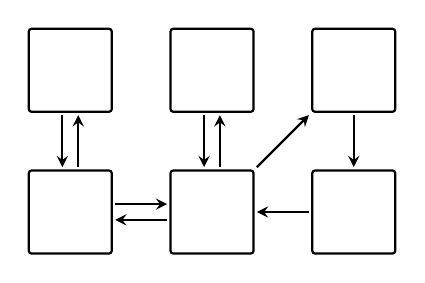
\begin{tikzpicture}[every node/.style={scale=3.0, draw=black, minimum width=10pt, minimum height=10pt, rounded corners=1},>=stealth, thick, node distance=0.6cm, rotate=90, transform shape]
        \node(modelo) at (0,0){};
        \node(banco) [right of=modelo]{};
        \node(controlador) [below of=modelo]{};
        \node(visualizacao) [right of=controlador]{};
        \node(roteador) [below of=controlador]{};
        \node(navegador) [right of=roteador]{};

        \draw[->] (modelo.-10) -- (banco.190);
        \draw[<-] (modelo.10) -- (banco.170);
        \draw[->] (modelo.-80) -- (controlador.80);
        \draw[<-] (modelo.-100) -- (controlador.100);
        \draw[->] (controlador.-10) -- (visualizacao.190);
        \draw[<-] (controlador.10) -- (visualizacao.170);
        \draw[->] (roteador) -- (controlador);
        \draw[->] (navegador) -- (roteador);
        \draw[->] (controlador) -- (navegador);
      \end{tikzpicture}
    \end{center}

  \pagebreak
  \vspace*{0.0cm}

  % SOURCES
  % - https://github.com/kumar91gopi/Algorithms-and-Data-Structures-in-Ruby
  % - https://github.com/djo/algorithms
  \item (1,8 pt) (a) Encontre o resultado do método a seguir para \textbf{array = [5, 1, 4, 2, 3]}; (b) Qual o propósito desse método? (c) Que linha deve ser alterada para que ele funcione da forma oposta?
  % (a) [1, 2, 3, 4, 5]
  % (b) ordenar um array em ordem crescente (algoritmo Selection Sort)
  % (c) linha 6, o ``<'' deve ser alterado para ``>'', de forma que o array ficará ordenado em ordem decrescente

    \begin{minted}[linenos=true]{ruby}
def metodo_misterioso(array)
  n = array.size - 1
  n.times do |i|
    min = i
    (i + 1).upto(n) do |j|
      min = j if array[j] < array[min]
    end
    if i != min
      temp = array[min]
      array[min] = array[i]
      array[i] = temp
    end
  end

  array
end
    \end{minted}
    \begin{itemize}[itemsep=0pt]
      \item [] \textbf{obs. 1:} o método \textbf{size} retorna o tamanho do array
      \item [] \textbf{obs. 2:} o método \textbf{times}, quando usado com um parâmetro de bloco, começa com 0 e vai até n - 1
    \end{itemize}

  % SOURCES
  % - https://github.com/kumar91gopi/Algorithms-and-Data-Structures-in-Ruby
  \item (1,8 pt) (a) Encontre o resultado do método a seguir para \textbf{array = (10..30).to\_a}, com \textbf{elem = 27} e \textbf{elem = 7}; (b) Qual o propósito desse método? (c) Ele funcionaria corretamente para \textbf{array = [4, 5, 10, 2, 8, 6, 3, 9, 1, 7]} e \textbf{elem = 6}?
  % (a) 17; ``Erro''
  % (b) buscar o índice de um certo elemento dentro do array (algoritmo de Busca Binária)
  % (c) não, o array deveria estar ordenado

  \begin{minted}{ruby}
def metodo_secreto(array, elem)
  inf = 0
  sup = array.length - 1

  while (inf <= sup)
    meio = (inf + sup) / 2

    if array[meio] == elem
      return meio
    elsif array[meio] < elem
      inf = meio + 1
    else
      sup = meio - 1
    end
  end

  return "Erro"
end
  \end{minted}
  \begin{itemize}[itemsep=0pt]
    \item [] \textbf{obs. 1:} o método \textbf{to\_a} transforma um range em um array
    \item [] \textbf{obs. 2:} o método \textbf{length} retorna o tamanho do array
    \item [] \textbf{obs. 3:} o operador \textbf{/} realiza a divisão inteira quando existe um número inteiro no denominador (ex.: 5 / 2 == 2; 5 / 2.0 == 2.5)
  \end{itemize}
\end{enumerate}
\end{multicols*}
\end{document}
